\documentclass{standalone}
\usepackage{tikz}
\standaloneenv{tikzpicture}
\usetikzlibrary{arrows}
\tikzset{%
 >=stealth'
}
\newenvironment{localtoimage}[3][]{%
 \node (I) [inner sep=0pt] {\includegraphics[#3]{#2}};%
 \begin{localto}[#1]{I}%
}{%
 \end{localto}%
}
\newenvironment{localto}[2][]{
 \path let \p1=(#2.center), \p2=(#2.north), \p3=(#2.east) in coordinate (#2X) at (\x3-\x1,0) coordinate (#2Y) at (0,\y2-\y1);
 \begin{scope}[x={(#2X)}, y={(#2Y)}, shift={(#2.center)},#1]
}{
 \end{scope}
}
\usepackage{substr}
% \def\jobname{dark}
\IfSubStringInString{\detokenize{dark}}{\jobname}{
%  \pagecolor{black}
 \def\fg{white}
 \def\bg{black}
 \color{\fg}
}{
 \def\fg{black}
 \def\bg{white}
}

\usetikzlibrary{positioning}
\begin{document}
\tikzset{%
 every node/.style={ultra thick},%
 wnode/.style={solid, draw=\fg},%
 snode/.style={draw=blue}%
}%
%
\def\visionimgs{0/0/000/start, 1/0/011/clue, 2/0/030/lure, 0/1/053/trap, 1/1/060/end}%
%
\begin{tikzpicture}[scale=.6]%
 \foreach \r/\c/\L in {2/snode/S, 1/wnode/W} {
  \foreach \a/\l in {0/e, 90/n, 180/w, 270/s} {
    \draw [\c, thick] (\a:\r) ++(-.5, -.5) rectangle ++(1, 1);
    \node at (\a:\r) {\footnotesize $\L_\l$};
  }
 }

 \node at (8, 0) {
  \begin{tabular}{rl}
   $W_*$ & Wall/Previous direction \\
   $S_*$ & Sign value (if any) \\
  \end{tabular}
 };
\end{tikzpicture}%
%
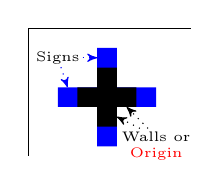
\begin{tikzpicture}
 \foreach \x/\y\step/\name in \visionimgs {
  \node (N\name) at (2.5*\x,-2.5*\y) [inner sep=0pt]
   {\includegraphics[width=2cm]{vision/dd/\step_\name}};
  \node [below=0 of N\name, inner sep=1pt] {\expandafter\MakeUppercase\name};
 }

 \begin{scope}[scale=.25, font=\footnotesize, shift={(19, -6)}]
  \draw (-3.5, -.5) -- ++(8.25, 0);
  \draw (-3.5, -.5) -- ++(0, -6.5);

  \fill [blue] (0, -1.5) rectangle ++(1, -5)
               (-2, -3.5) rectangle ++(5, -1);
  \fill [\fg]  (0, -2.5) rectangle ++(1, -3)
               (-1, -3.5) rectangle ++(3, -1);
  \fill [\bg]  (0, -3.5) rectangle ++(1, -1);

  \node (S) [inner sep=1pt] at (-2, -2) {\tiny Signs};
  \draw [->, dotted, blue] (S) -- (0, -2);
  \draw [->, dotted, blue] (S) -- (-1.5, -3.5);

  \node (W) [inner sep=1pt] at (3, -6) {\tiny Walls or};
  \node [below=0 of W, inner sep=1pt, red] {\tiny Origin};
  \draw [->, dotted] (W) -- (1.5, -4.5);
  \draw [->, dotted] (W) -- (1, -5);

 \end{scope}

\end{tikzpicture}%
%
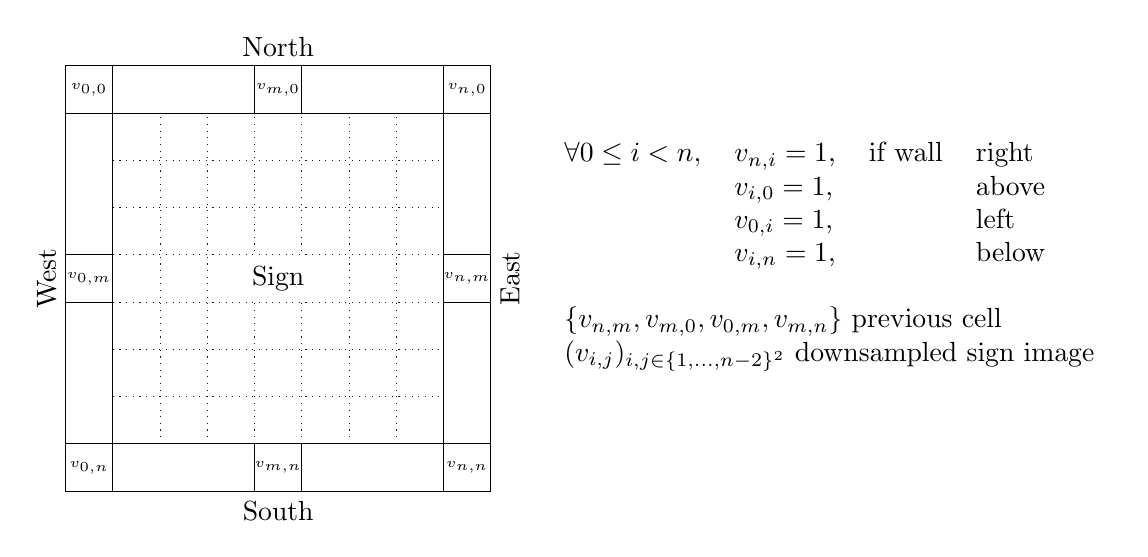
\begin{tikzpicture}[scale=.6, y=-1cm]
 \draw [dotted] (1,1) grid (8,8);
 \fill [opacity=.1, white] (1,1) rectangle (8,8) node [pos=.5, opacity=1, black, fill=white] {Sign};
 \draw (0,0) rectangle (9,1) node at (4.5,9) [anchor=north] {South};
 \draw (0,0) rectangle (1,9) node at (0,4.5) [anchor=south, rotate=90] {West};
 \draw (8,0) rectangle (9,9) node at (9,4.5) [anchor=north, rotate=90] {East};
 \draw (0,8) rectangle (9,9) node at (4.5,0) [anchor=south] {North};
 \def\hn{m}
 \foreach \x/\y/\i/\j in {0/0/0/0, 0/8/0/n, 8/0/n/0, 8/8/n/n,
                          4/0/\hn/0, 0/4/0/\hn, 4/8/\hn/n, 8/4/n/\hn} {
  \node at (\x+.5, \y+.5) {\tiny $v_{\i,\j}$};
  \draw (\x,\y) rectangle ++(1,1);
 }

 \node at (10, 4) [anchor=west] {
  \begin{tabular}{llll}
   $\forall 0\leq i < n,$\ & $v_{n,i} = 1$, & if wall & right \\
                           & $v_{i,0} = 1$, &         & above \\
                           & $v_{0,i} = 1$, &         & left \\
                           & $v_{i,n} = 1$, &         & below \\
   \\
   \multicolumn{4}{l}{$\{v_{n,m}, v_{m,0}, v_{0,m}, v_{m,n}\}$ previous cell}\\
   \multicolumn{4}{l}{$(v_{i,j})_{i,j \in \{1,...,n-2\}^2}$ downsampled sign image}
  \end{tabular}
 };
\end{tikzpicture}%
%
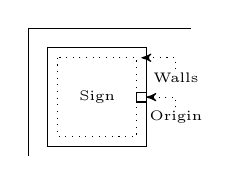
\begin{tikzpicture}%
 \foreach \x/\y\step/\name in \visionimgs {
  \node (N\name) at (2.5*\x,-2.5*\y) [inner sep=0pt, draw=black]
   {\includegraphics[width=2cm]{vision/cd/\step_\name}};
  \node [below=0 of N\name, inner sep=1pt] {\expandafter\MakeUppercase\name};
 }

 \begin{scope}[scale=.25, font=\footnotesize, shift={(19, -6)}]
  \draw (-3.5, -.5) -- ++(8.25, 0);
  \draw (-3.5, -.5) -- ++(0, -6.5);
  \draw (-2.5, -1.5) rectangle ++(5, -5);
  \draw [dotted] (-2, -2) rectangle ++(4, -4);
  \node at (0, -4) {\tiny Sign};
  \node [inner sep=1pt] (W) at (4, -3) {\tiny Walls};
  \node [inner sep=1pt] (O) at (4, -5) {\tiny Origin};
  \fill [draw=\fg, fill=white] (2, -4.25) rectangle ++(.5, .5);
  \draw [dotted, ->] (W) |- (2.25, -2);
  \draw [dotted, ->] (O) |- (2.5, -4);
 \end{scope}

\end{tikzpicture}%
%
\end{document}
